\begin{figure}
\centering
\subfloat[Straddling]{
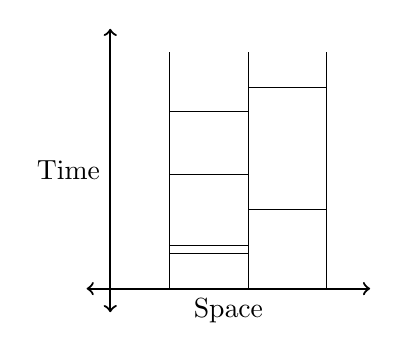
\begin{tikzpicture}
    \draw[<->,thick] (-0.3,0)--(3.3,0) node[midway,below] {Space};
    \draw[<->,thick] (0,-0.3)--(0,3.3) node[midway,left] {Time};
    \draw[-] (0.75,0)--(0.75,3);
    \draw[-] (1.75,0)--(1.75,3);
    \draw[-] (2.75,0)--(2.75,3);
    \draw[-] (0.75, 0.45)--(1.75, 0.45);
    \draw[-] (0.75, 0.55)--(1.75, 0.55);
    \draw[-] (0.75, 1.45)--(1.75, 1.45);
    \draw[-] (0.75, 2.25)--(1.75, 2.25);
    \draw[-] (1.75, 1)--(2.75, 1);
    \draw[-] (1.75, 2.55)--(2.75, 2.55);
\end{tikzpicture}
}\hspace{1in}
\subfloat[Locally Ordered]{
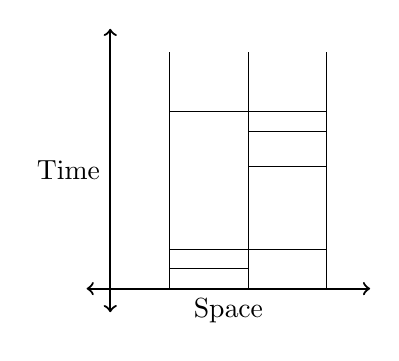
\begin{tikzpicture}
    \draw[<->,thick] (-0.3,0)--(3.3,0) node[midway,below] {Space};
    \draw[<->,thick] (0,-0.3)--(0,3.3) node[midway,left] {Time};
    \draw[-] (0.75,0)--(0.75,3);
    \draw[-] (1.75,0)--(1.75,3);
    \draw[-] (2.75,0)--(2.75,3);
    \draw[-] (0.75, 0.25)--(1.75, 0.25);
    \draw[-] (0.75, 0.5)--(1.75, 0.5);
    \draw[-] (0.75, 2.25)--(1.75, 2.25);
    \draw[-] (1.75, 0.5)--(2.75, 0.5);
    \draw[-] (1.75, 1.55)--(2.75, 1.55);
    \draw[-] (1.75, 2)--(2.75, 2);
    \draw[-] (1.75, 2.25)--(2.75, 2.25);
\end{tikzpicture}
}
\caption{Comparison of two event traces.}
\label{fig:sol-cartoon}
\end{figure}